\documentclass[12pt]{article}
\usepackage{amsmath}
\usepackage[margin=2.5cm]{geometry}
\usepackage[utf8]{inputenc}
\usepackage{amsfonts}
\usepackage{fancyhdr}
\usepackage{hyperref}
\usepackage{graphicx}
\usepackage{caption}
\usepackage{subcaption}
\usepackage{setspace}
\usepackage{float}
\usepackage{svg}
\setstretch{1.3} 
\usepackage{array}
\usepackage {xcolor}
%...

\usepackage{multirow} % Required for multirows




%...

%\usepackage{csc}% unknown package
\pagestyle{fancy}
\fancyhead[L]{Denoising of Signals and Photo with Wavelet}
\fancyhead[R]{Page \thepage}
\fancypagestyle{firstpage}{%
  \lhead{}
  \rhead{}
}

\begin{document}
\begin{figure*}[!tbp]
  \begin{subfigure}[b]{0.2 \textwidth}
    
\includegraphics[width=\textwidth]{img/uni}
  \end{subfigure}
  \hfill
  \begin{subfigure}[b]{0.25\textwidth}
    
\includegraphics[width=\textwidth]{img/fani}
  \end{subfigure}
\end{figure*}
\begin{center}
\textbf{Denoising of Signals and Photo with Wavelet} \\[1in]
Professor : Dr. Safari\\~\\
St : AmirAbbas Saberi
\\[4in]
\textbf{University of Tehran}\\
May,15,2023
\end{center}
	\thispagestyle{firstpage}
\newpage
If our ear uses a certain technique to analyze a signal, then if
you use that same mathematical technique, you will be doing
something like our ear. You might miss important things, but
you would miss things that our ear would miss too.
 \begin{flushright}
 \textit{Ingrid Daubechies}
  \end{flushright} 
 The mathematical analysis of the frequency content of signals is called
Fourier analysis. 
analysis as it applies to discrete signals and use it to analyze the frequency
content of wavelets. A deeper understanding of wavelets can be gained from
studying their frequency content, and by examining how this frequency
content relates to wavelet transforms of signals.  \\
To understand better the mathematics
as simple as possible we shall focus on 1D signals.then we concetrate on photos(2D signals).The main Philosophy of generating of wavelet is defects in Statical feature of time or space Fourier analysis.\\
The aim of doing this project is to remove noise as possible as can.

\section{1D Wavelet:}
First, we need to create pure siganl without any noise with some asumpptions that i will say as follows :\\
1- $ f =  2cos( {8 \pi x}/N ) + {4 \pi x}/N$\\
2- N = Numbers of sample of signals we have : $2^n$ \\
we consider n = 8.

\begin{figure}[h]
    \centering
    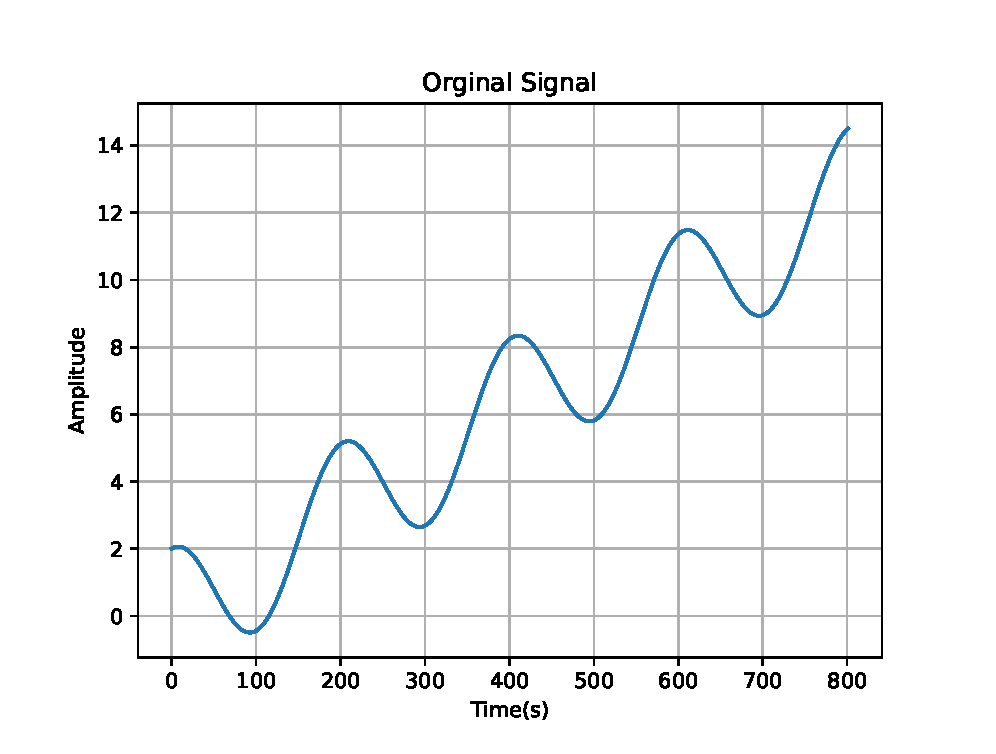
\includegraphics[width=0.6\textwidth]{img/Harr_org.eps}
    \caption{Orginal 1D signals $2cos( {8 \pi x}/N ) + {4 \pi x}/N$}
    \label{fig:mesh1}
\end{figure}
\newpage
Then we add sum noise(Random Gaussian Noise) to make a noisy signals : 
\begin{figure}[h]
    \centering
    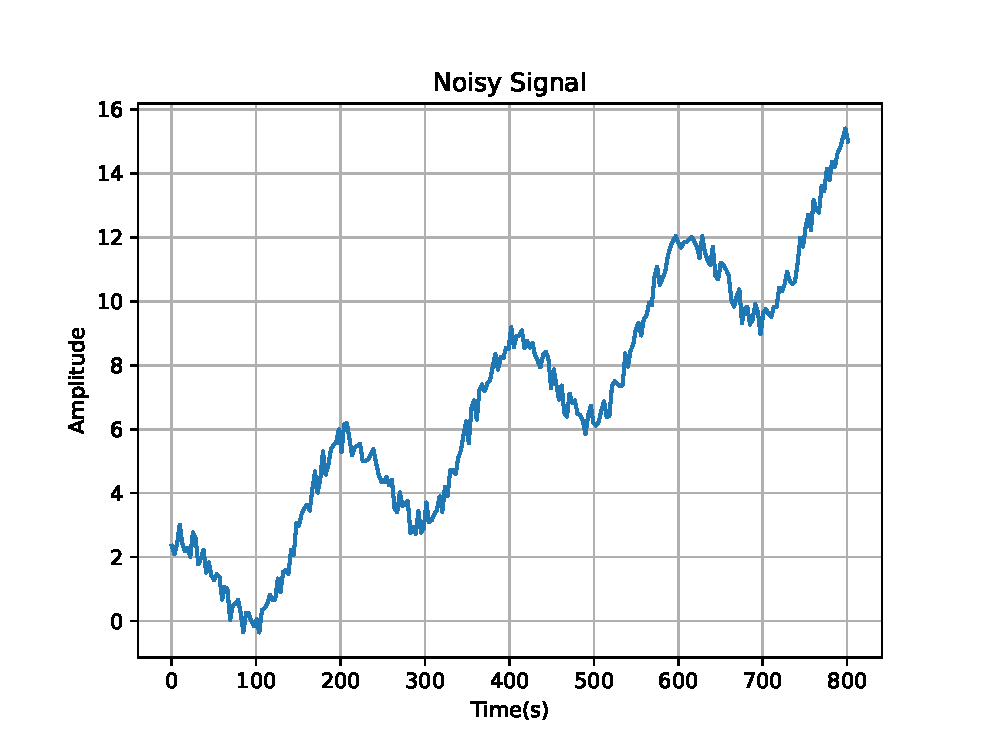
\includegraphics[width=0.6\textwidth]{img/Noisy_Signal.eps}
    \caption{Noisy 1D signals $2cos( {8 \pi x}/N ) + {4 \pi x}/N + random_{noise}$}
    \label{fig:mesh1}
\end{figure}
main strucure of wavelet is finding some cofficeint to recreate our signal without noise :
\[ f =\sum\limits_{i=1} \langle f \; , \; v^1_{i} \rangle v^1_{i} +  \sum\limits_{j=1}^{\frac{N}{2^j}}\sum\limits_{i=1}  \langle f \; , \; w^j_{i} \rangle w^j_{i} \] \\
Here we use some type of wavewlet like Harr ,Daubechies and Mexician Hat which is in order write as follows : 
\newpage
\subsection{Harr 1D:}
firse we write scale functions and creator function of Harr and then we seprate signals in to Avrage part and Details part with these function.\\
\begin{equation}
  \phi(x)=\begin{cases}
    1, & \text{if $0 \le x<1$}.\\
    0, & \text{otherwise}.
  \end{cases}
\end{equation} 

\begin{equation}
  \psi(x)=\begin{cases}
    1, & \text{if $0 \le x<1/2$}.\\
    
    -1, & \text{if $1/2 \le x<1$}.\\
    0, & \text{otherwise}.
  \end{cases}
\end{equation}
and the result is :\\
\begin{figure}[h]
    \centering
    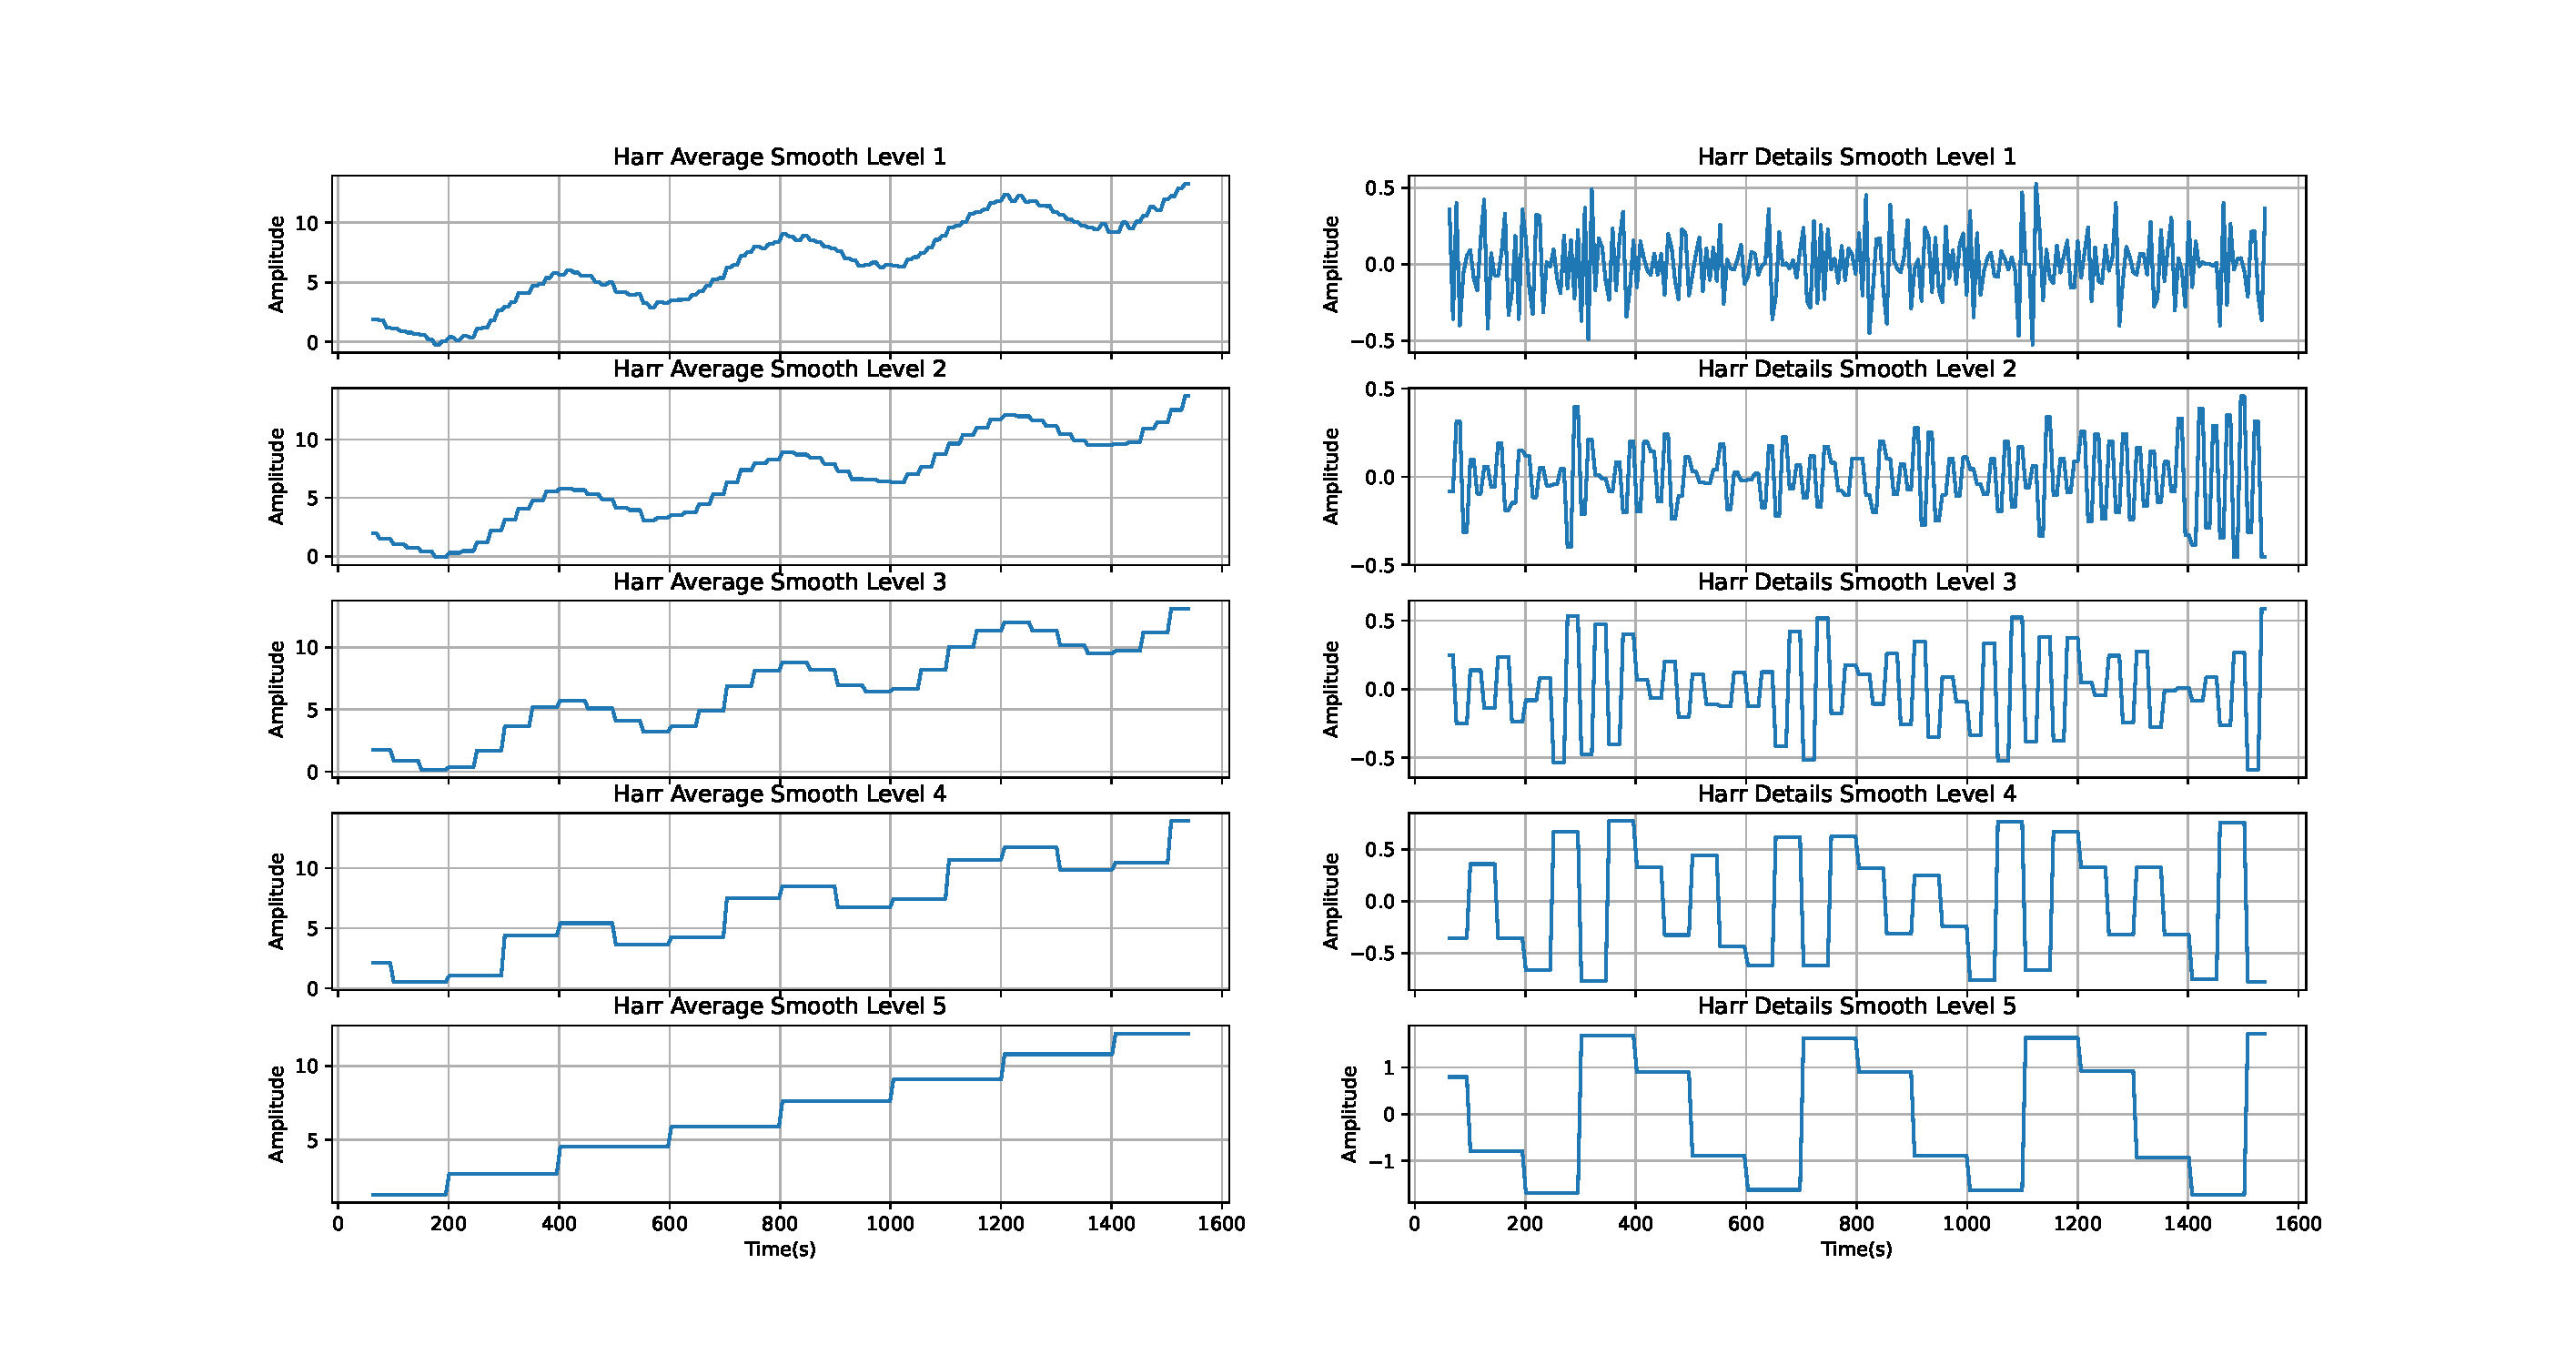
\includegraphics[width=1.1\textwidth]{img/Harr.eps}
    \caption{Harr Wavelet level1 to level5}
    \label{fig:mesh1}
\end{figure}
\newpage
\subsection{Daubechies4 1D:}
cofficent is root of recreating function with wavelet method and for Daubechies4 is given as follows : \\


\centerline{
\begin{tabular}{llll}
$\alpha_1 = \frac{1+\sqrt{3}}{4\sqrt{2}}$ & $\alpha_2 = \frac{3+\sqrt{3}}{4\sqrt{2}}$ & $\alpha_3 = \frac{3-\sqrt{3}}{4\sqrt{2}}$ &  $\alpha_4 = \frac{1-\sqrt{3}}{4\sqrt{2}}$ 
\end{tabular}}

\centerline{
\begin{tabular}{l}
$v_1^1 = (\alpha_1,\alpha_2,\alpha_3,\alpha_4,0,0,0,0...,0)$\\
$v_1^2 = (0,0,\alpha_1,\alpha_2,\alpha_3,\alpha_4,0,0,...0)$\\
.\\
.\\
.\\
$v_{\frac{N}{2}}^2 = (\alpha_3,\alpha_4,0,0,0,0,...0,\alpha_1,\alpha_2)$\\
\end{tabular}}

\centerline{
\begin{tabular}{llll}
$\beta_1 = \frac{1+\sqrt{3}}{4\sqrt{2}}$ & $\beta_2 = \frac{3+\sqrt{3}}{4\sqrt{2}}$ & $\beta_3 = \frac{3-\sqrt{3}}{4\sqrt{2}}$ &  $\beta_4 = \frac{1-\sqrt{3}}{4\sqrt{2}}$ 
\end{tabular}}

\centerline{
\begin{tabular}{l}
$w_1^1 = (\beta_1,\beta_2,\beta_3,\beta_4,0,0,0,0...,0)$\\
$w_1^2 = (0,0,\beta_1,\beta_2,\beta_3,\beta_4,0,0,...0)$\\
.\\
.\\
.\\
$w_{\frac{N}{2}}^2 = (\beta_3,\beta_4,0,0,0,0,...0,\beta_1,\beta_2)$\\
\end{tabular}}

\begin{center}
$v^{n+1}_m = \alpha_1 v^n_{2m-1} + \alpha_2 v^n_{2m} + \alpha_3 v^n_{2m+1} + \alpha_4 v^n_{2m+2}$\\
$w^{n+1}_m = \beta_1 w^n_{2m-1} + \beta_2 w^n_{2m} + \beta_3 w^n_{2m+1} + \beta_4 w^n_{2m+2}$
\end{center}
\begin{equation}
  v^1_n . v^1_m=\begin{cases}
    1, & \text{if $m = n$}.\\
    
    0, & \text{if $m \neq n $}
  \end{cases}
\end{equation}
\begin{equation}
  w^1_n . w^1_m=\begin{cases}
    1, & \text{if $m = n$}.\\
    
    0, & \text{if $m \neq n $}
  \end{cases}
\end{equation}
\begin{equation}
  w^1_n . w^1_m = 0 , n,m \in Z
\end{equation}
\newpage
and the result is :\\
\begin{figure}[h]
    \centering
    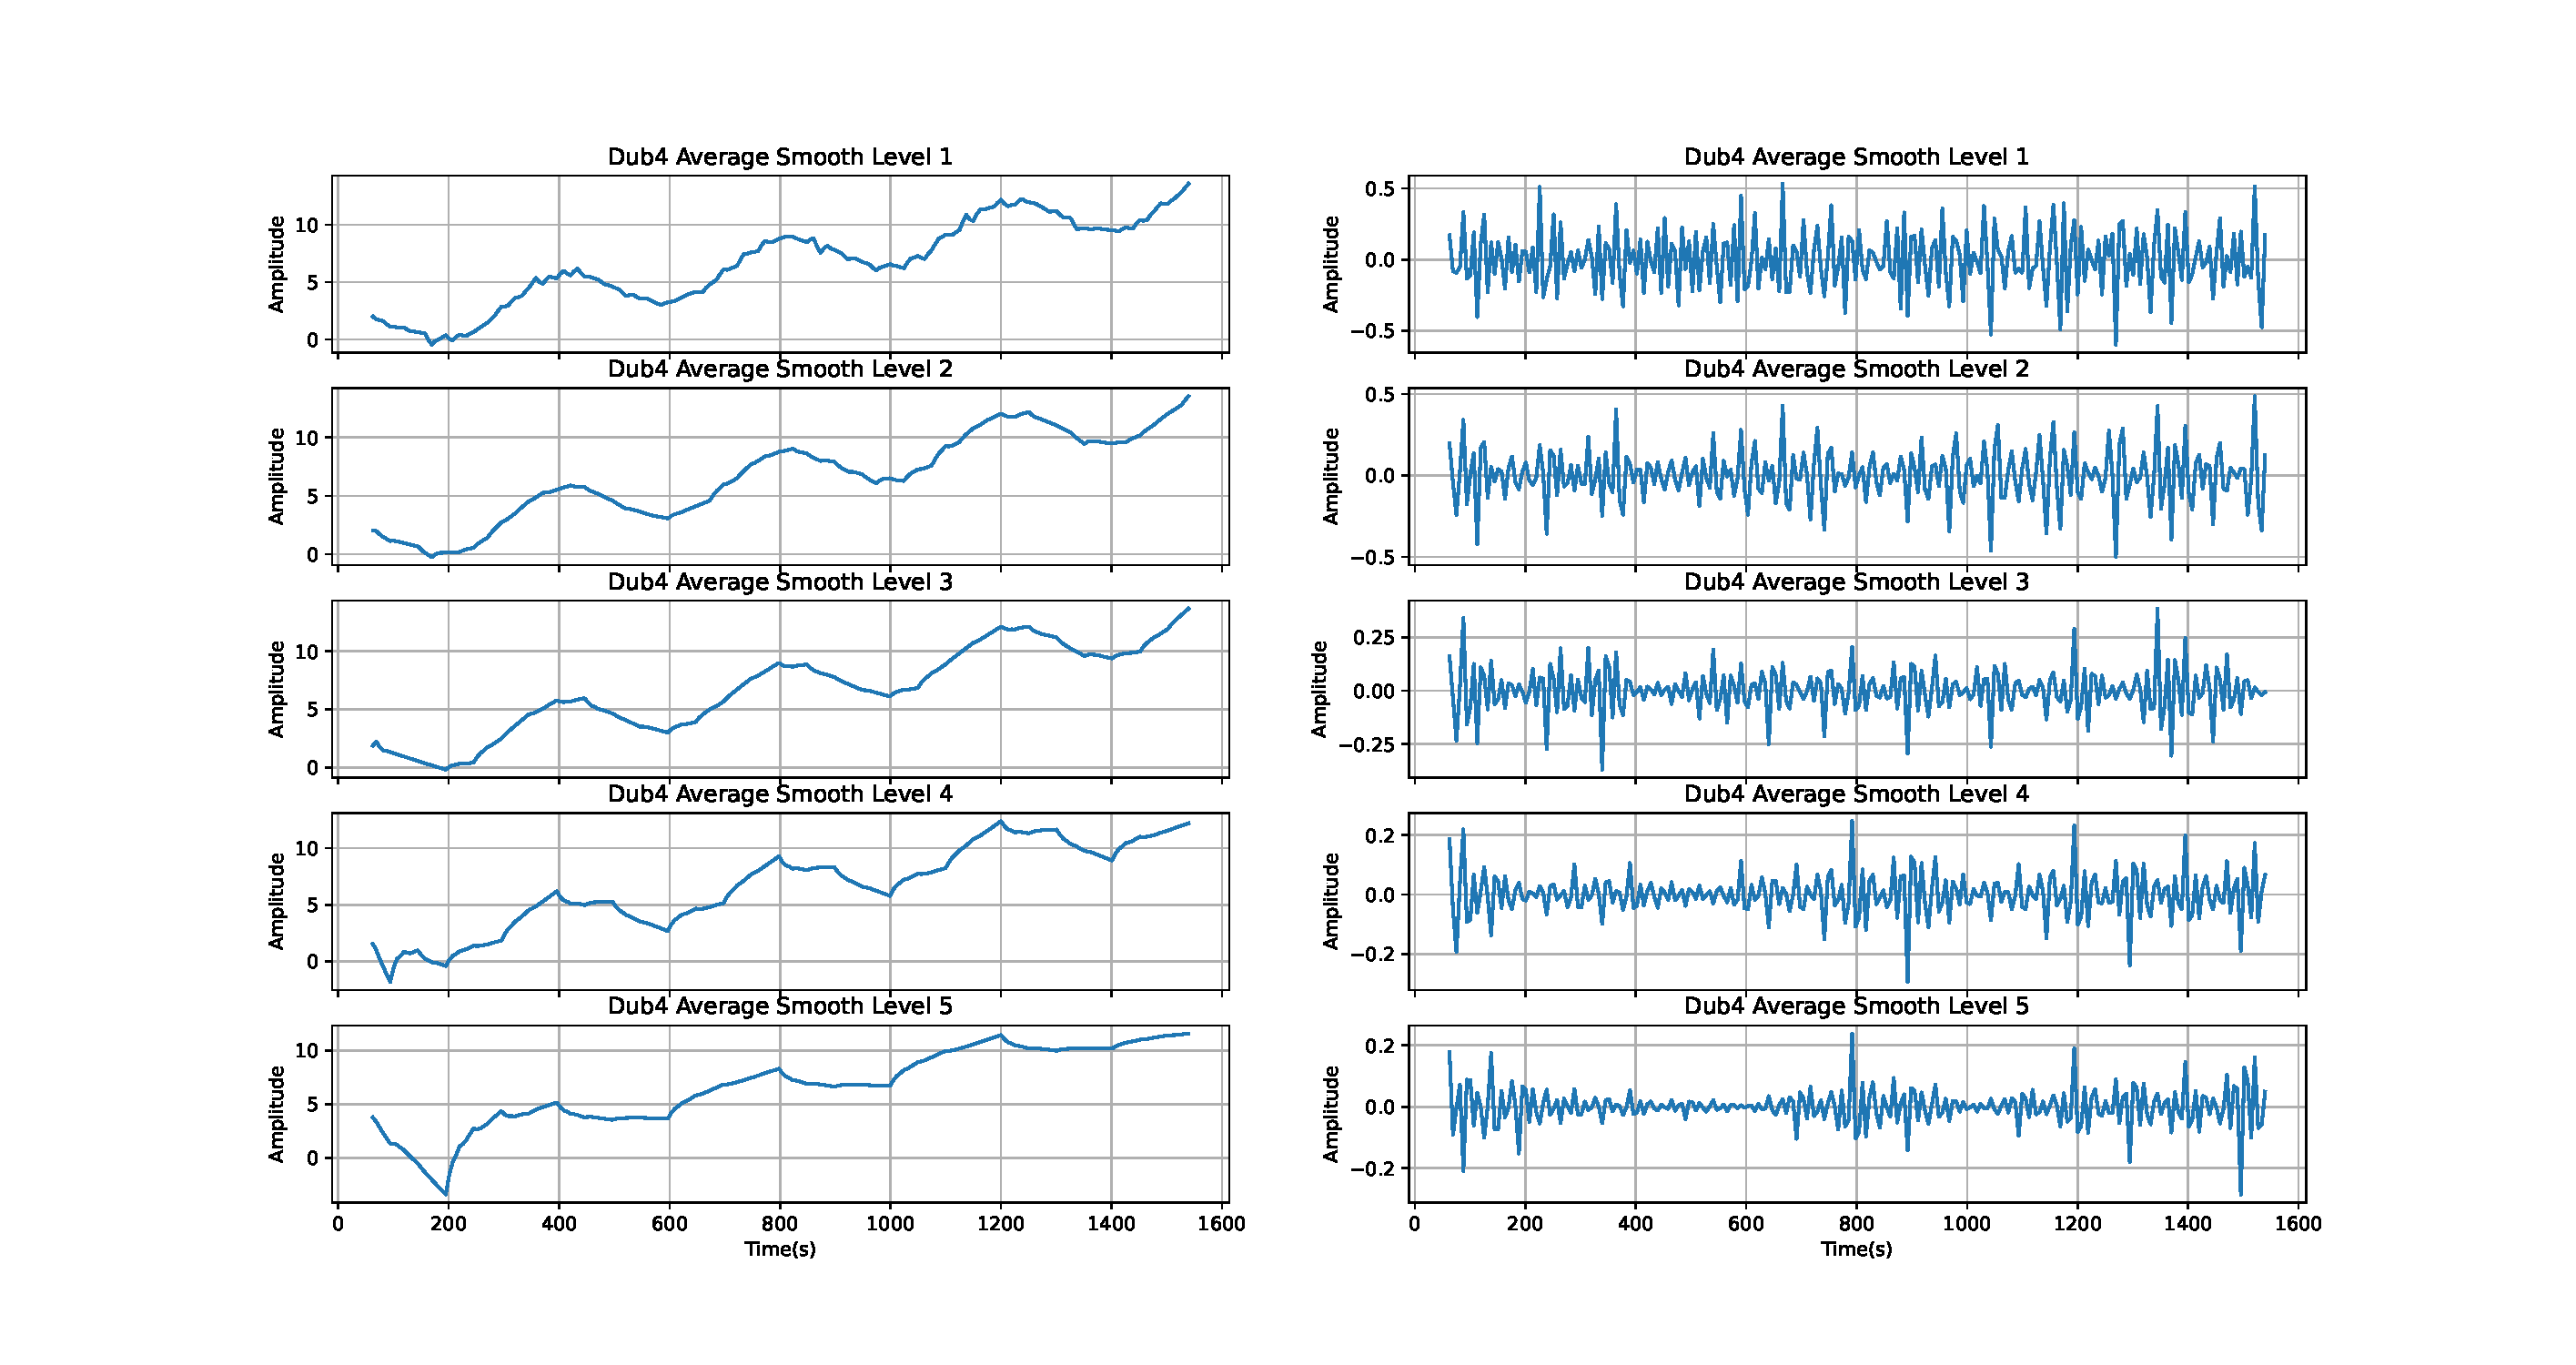
\includegraphics[width=1.1\textwidth]{img/Dub4.eps}
    \caption{Daubechies4 Wavelet level1 to level5}
    \label{fig:mesh1}
\end{figure}
\newpage
\subsection{Daubechies6 1D:}
cofficent is root of recreating function with wavelet method and for Daubechies4 is given as follows : \\


\centerline{
\begin{tabular}{llllll}
$\alpha_1 = 0.33267$ & $\alpha_2 = 0.80689$ & $\alpha_3 = 0.45987$ &  $\alpha_4 = -0.13501$ &  $\alpha_5 = -0.08544$ &  $\alpha_6 = 0.03522$ 
\end{tabular}}

\centerline{
\begin{tabular}{l}
$v_1^1 = (\alpha_1,\alpha_2,\alpha_3,\alpha_4,\alpha_5,\alpha_6,0,0,0,0...,0)$\\
$v_1^2 = (0,0,\alpha_1,\alpha_2,\alpha_3,\alpha_4,\alpha_5,\alpha_6,0,0,...0)$\\
.\\
.\\
.\\
$v_{\frac{N}{2}}^2 = (\alpha_3,\alpha_4,\alpha_5,\alpha_60,0,0,0,...0,\alpha_1,\alpha_2)$\\
\end{tabular}}

\centerline{
\begin{tabular}{llllll}
$\beta_1 = \alpha_6$ & $\beta_2 = -\alpha_5$ & $\beta_3 = \alpha_4$ &  $\beta_4 = -\alpha_3 $ &  $\beta_5 = \alpha_2 $  &  $\beta_6 = -\alpha_1 $ 
\end{tabular}}

\centerline{
\begin{tabular}{l}
$w_1^1 = (\beta_1,\beta_2,\beta_3,\beta_4,\beta_5,\beta_6,0,0,0,0...,0)$\\
$w_1^2 = (0,0,\beta_1,\beta_2,\beta_3,\beta_4,\beta_5,\beta_6,0,0,...0)$\\
.\\
.\\
.\\
$w_{\frac{N}{2}}^2 = (\beta_3,\beta_4,\beta_5,\beta_6,0,0,0,0,...0,\beta_1,\beta_2)$\\
\end{tabular}}

\begin{center}
$v^{n+1}_m = \alpha_1 v^n_{2m-1} + \alpha_2 v^n_{2m} + \alpha_3 v^n_{2m+1} + \alpha_4 v^n_{2m+2} + \alpha_5 v^n_{2m+3} + \alpha_6 v^n_{2m+4}$\\
$w^{n+1}_m = \beta_1 w^n_{2m-1} + \beta_2 w^n_{2m} + \beta_3 w^n_{2m+1} + \beta_4 w^n_{2m+2} + \beta_5 w^n_{2m+3} + \beta_6 w^n_{2m+4}$
\end{center}
\begin{equation}
  v^1_n . v^1_m=\begin{cases}
    1, & \text{if $m = n$}.\\
    
    0, & \text{if $m \neq n $}
  \end{cases}
\end{equation}
\begin{equation}
  w^1_n . w^1_m=\begin{cases}
    1, & \text{if $m = n$}.\\
    
    0, & \text{if $m \neq n $}
  \end{cases}
\end{equation}
\begin{equation}
  w^1_n . w^1_m = 0 , n,m \in Z
\end{equation}
\newpage
and the result is :\\
\begin{figure}[h]
    \centering
    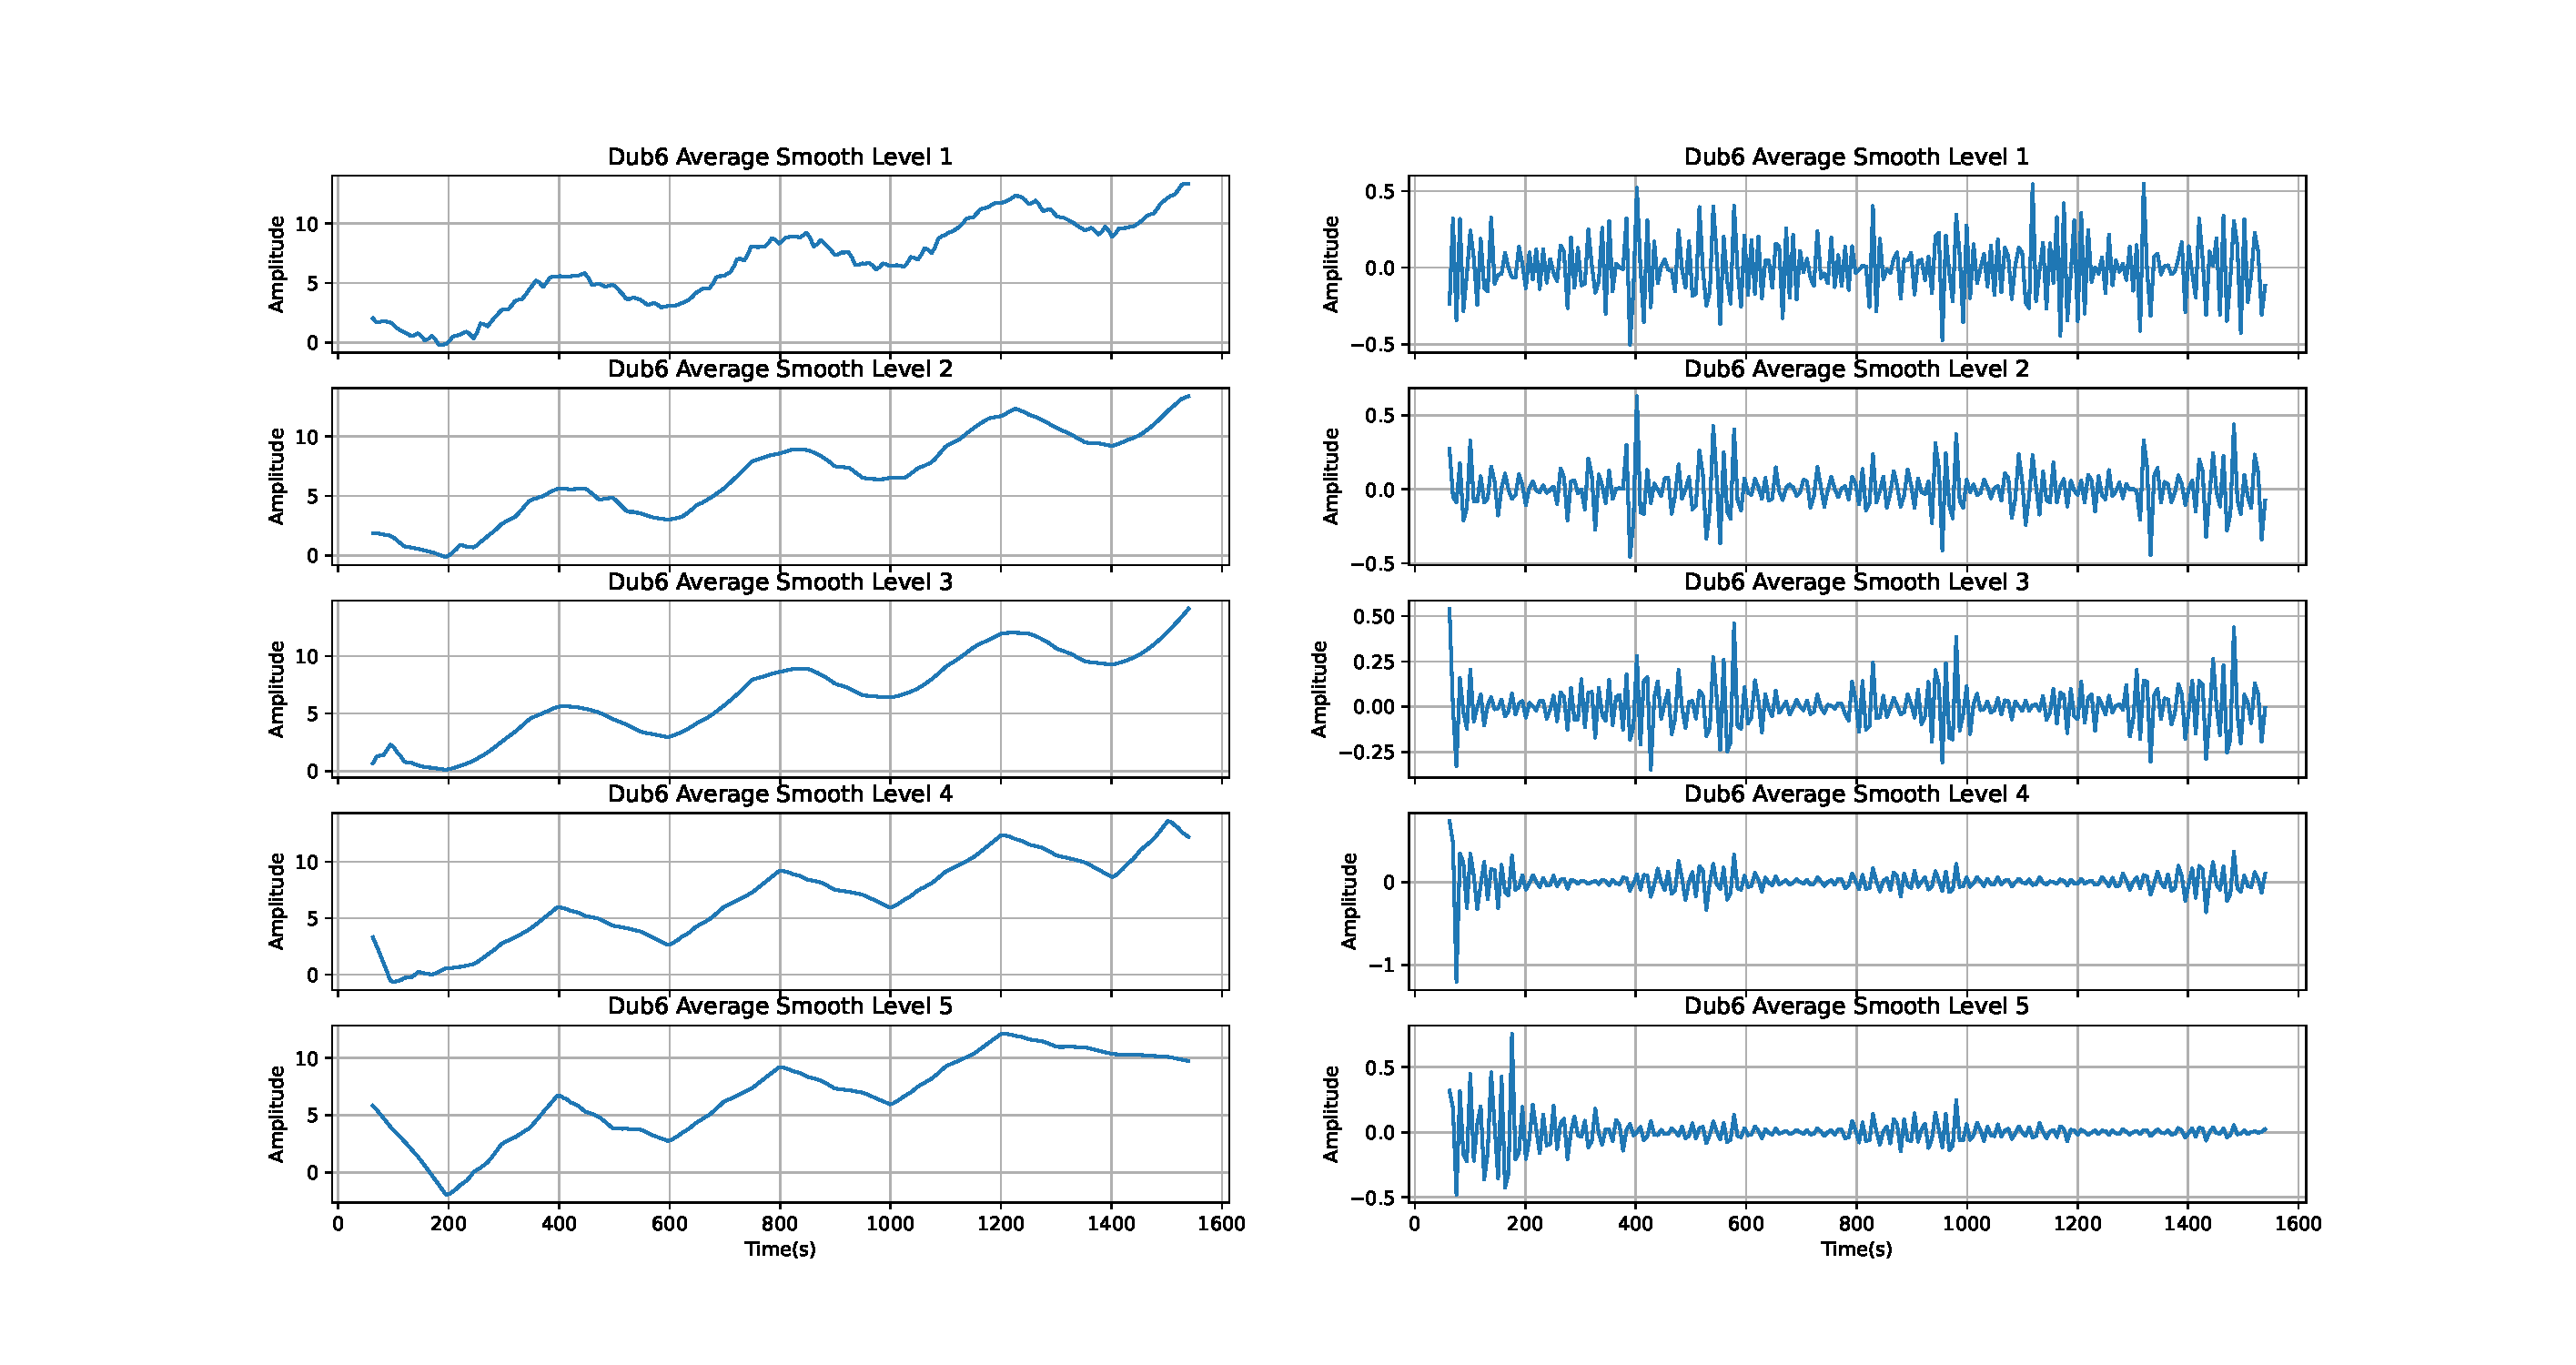
\includegraphics[width=1.1\textwidth]{img/Dub6.eps}
    \caption{Daubechies6 Wavelet level1 to level5}
    \label{fig:mesh1}
\end{figure}
\newpage
\subsection{Mexician Hat 1D:}
There is any different between Daubechies6 and Mexician Hat except , difference in cofficent  : \\


\centerline{
\begin{tabular}{llllll}
$\alpha_1 = \frac{1-\sqrt{7}}{16\sqrt{2}}$ & $\alpha_2 = \frac{5+\sqrt{7}}{16\sqrt{2}}$ & $\alpha_3 = \frac{14+2\sqrt{7}}{16\sqrt{2}}$ &  $\alpha_4 = \frac{14-2\sqrt{7}}{16\sqrt{2}}$ &  $\alpha_5 = \frac{1-\sqrt{7}}{16\sqrt{2}}$ &  $\alpha_6 = \frac{-3+\sqrt{7}}{16\sqrt{2}}$ 
\end{tabular}}



\centerline{
\begin{tabular}{llllll}
$\beta_1 = \alpha_6$ & $\beta_2 = -\alpha_5$ & $\beta_3 = \alpha_4$ &  $\beta_4 = -\alpha_3 $ &  $\beta_5 = \alpha_2 $  &  $\beta_6 = -\alpha_1 $ 
\end{tabular}}



and the result is :\\
\begin{figure}[h]
    \centering
    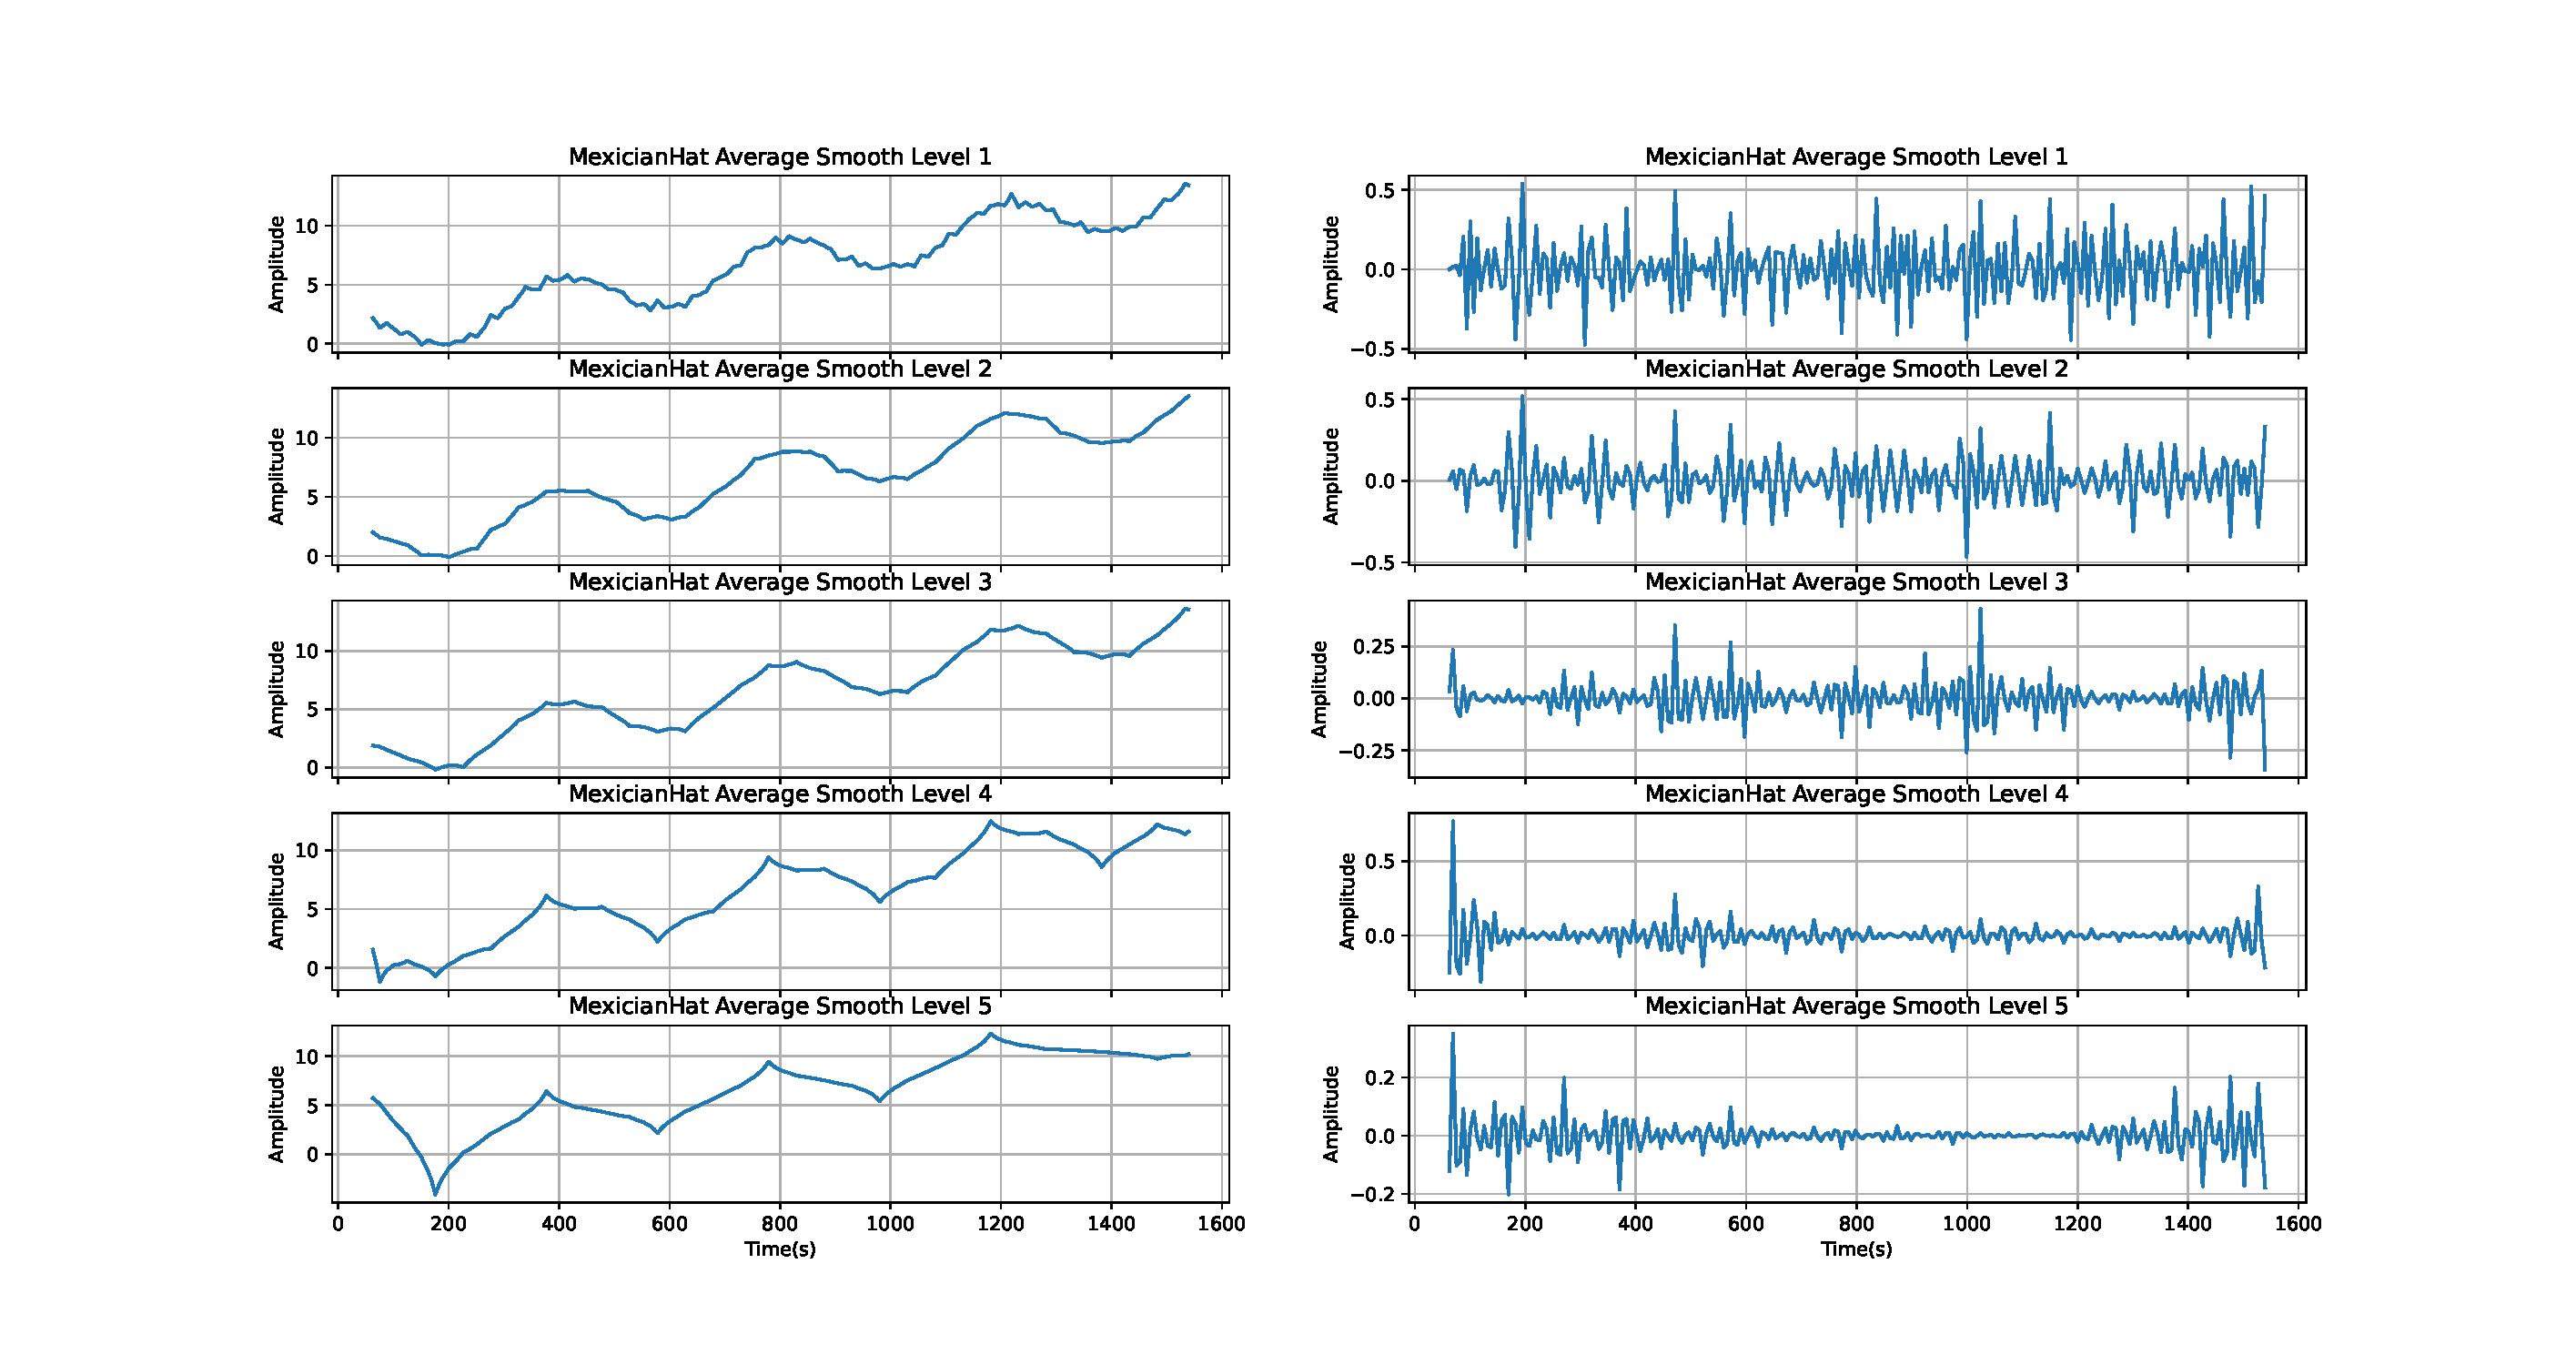
\includegraphics[width=1.1\textwidth]{img/Mex.eps}
    \caption{Mexician Hat Wavelet level1 to level5}
    \label{fig:mesh1}
\end{figure}
\newpage
\subsection{Conclution 1D Wavelet :}

\begin{equation}
e = \Sigma (f^i - f_w^i)^2
\end{equation}

\begin{table}[h!]
  \begin{center}
    \caption{Table of Wavelet Error.}
    \label{tab:table1}
    \begin{tabular}{c|c|c|c}
      \multicolumn{4}{c}{Wavelet}\\
      \hline
      \multirow{2}{*}{Harr} & \multirow{2}{*}{Dub6} & \multirow{2}{*}{Dub4} & \multirow{2}{*}{Mexicain Hat}\\ 
      & & & \\
      \hline
      \color{green} 67.6701 & 64.8833 & 71.8755 & 61.5979 \\
      67.7504 & \color{green}60.8257 & \color{green}66.38971 & 56.0953 \\
      81.7307 & 62.0543 & 66.4861 & \color{green}54.8403 \\
      153.601 & 94.8377 & 104.948 & 86.0585 \\
      584.675 & 176.142 & 317.073 & 183.6669
      
    \end{tabular}
  \end{center}
\end{table}
Level three of Mexician Hat is the best in our sample.
\newpage

\section{2D Wavelet:}
Asump an image N*N . level of this image represents below :\\
\begin{center}
$f \rightarrow \begin{pmatrix}
aa^1 & ad^1 \\ 
da^1 & dd^1
\end{pmatrix} \rightarrow ... \rightarrow \begin{pmatrix}
aa^m & ad^m \\ 
da^m & dd^m
\end{pmatrix} 
$
\end{center}
In here the base element of our space caculte from this formula :\\
\begin{equation}
V^1_{11} \otimes W^1_{11} = (V^1_{11})^T W^1_{11} 
\end{equation}
so we have :
\begin{equation}
f = aa_{11}^j V^1_{11} \otimes V^1_{11} + .... + aa_{N/2 M/2}^j V^1_{N/2 M/2} \otimes V^1_{N/2 M/2} \\
+ dd_{11}^j W^1_{11} \otimes W^1_{11} + .... + dd_{N/2 M/2}^j W^1_{N/2 M/2} \otimes W^1_{N/2 M/2}
\end{equation}
now we consider an image here : 

\begin{figure}[h]
    \centering
    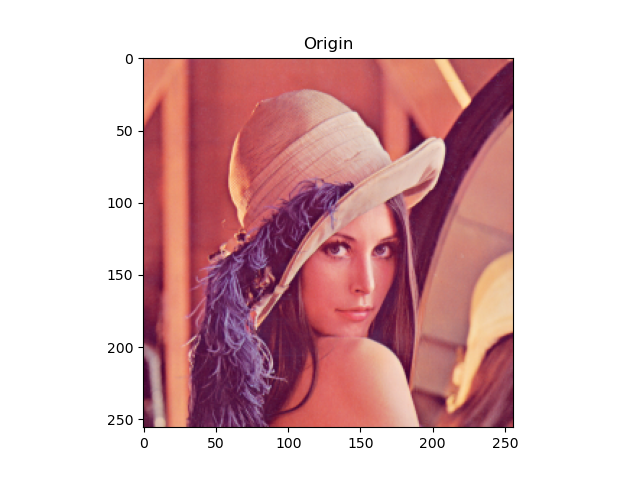
\includegraphics[width=0.8\textwidth]{img/lena.png}
    \caption{The Orginal image without any noise}
    \label{fig:mesh1}
\end{figure}
\newpage
Then we put some noise in it : 

\begin{figure}[h]
    \centering
    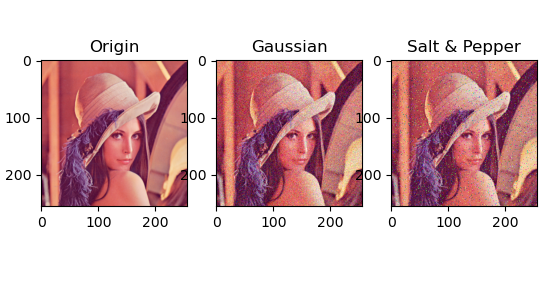
\includegraphics[width=0.8\textwidth]{img/LenaNoise.png}
    \caption{The Orginal image pluse gaussian noise and salt and pepper noise}
    \label{fig:mesh1}
\end{figure}

\subsection{Harr 2D :}
\begin{figure}[h]
    \centering
    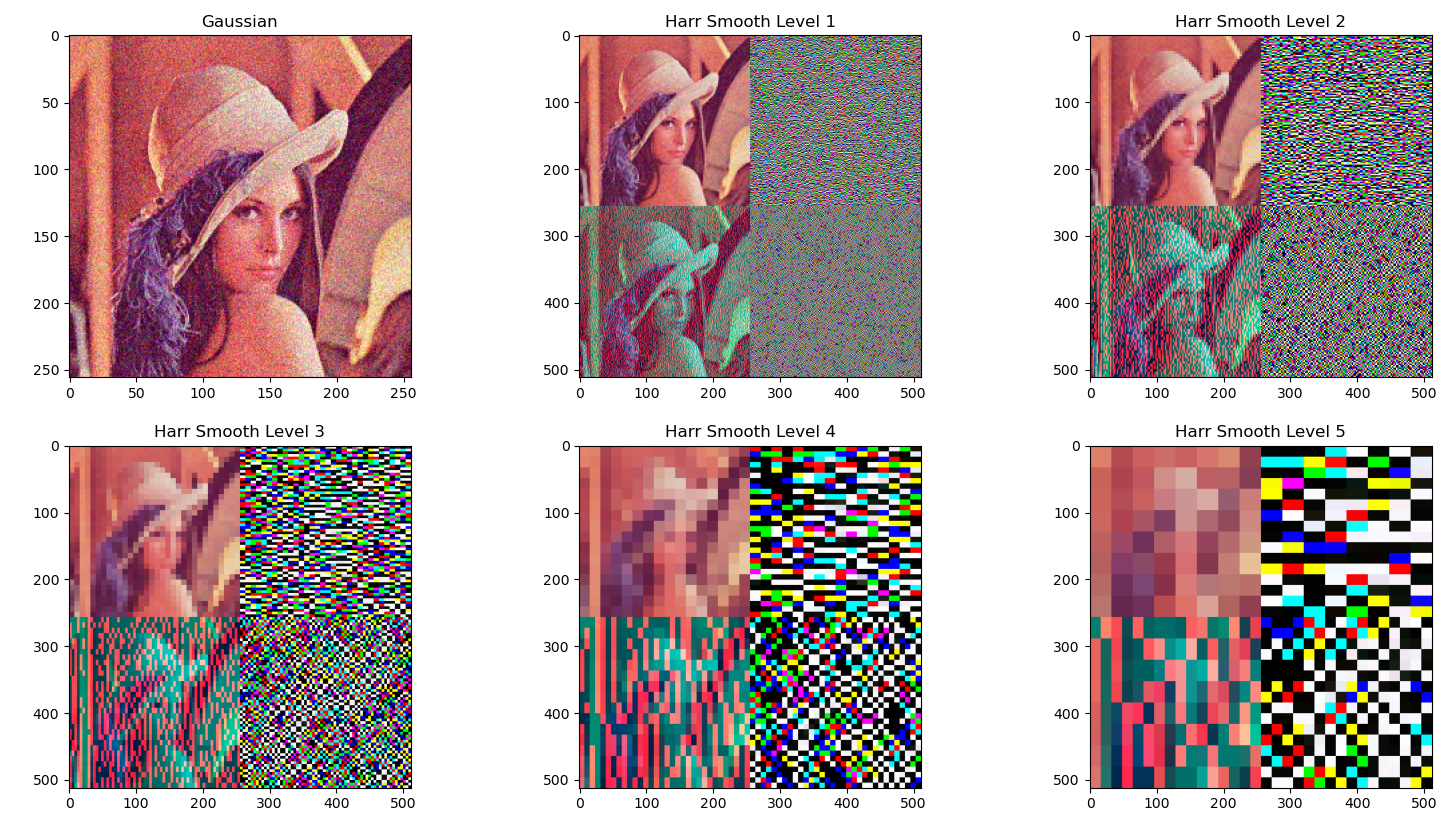
\includegraphics[width=0.8\textwidth]{img/Lena_Harr.png}
    \caption{Harr 2D Wavelet level1 to level5}
    \label{fig:mesh1}
\end{figure}
\newpage
\subsection{Daubechies4 2D :}
\begin{figure}[h]
    \centering
    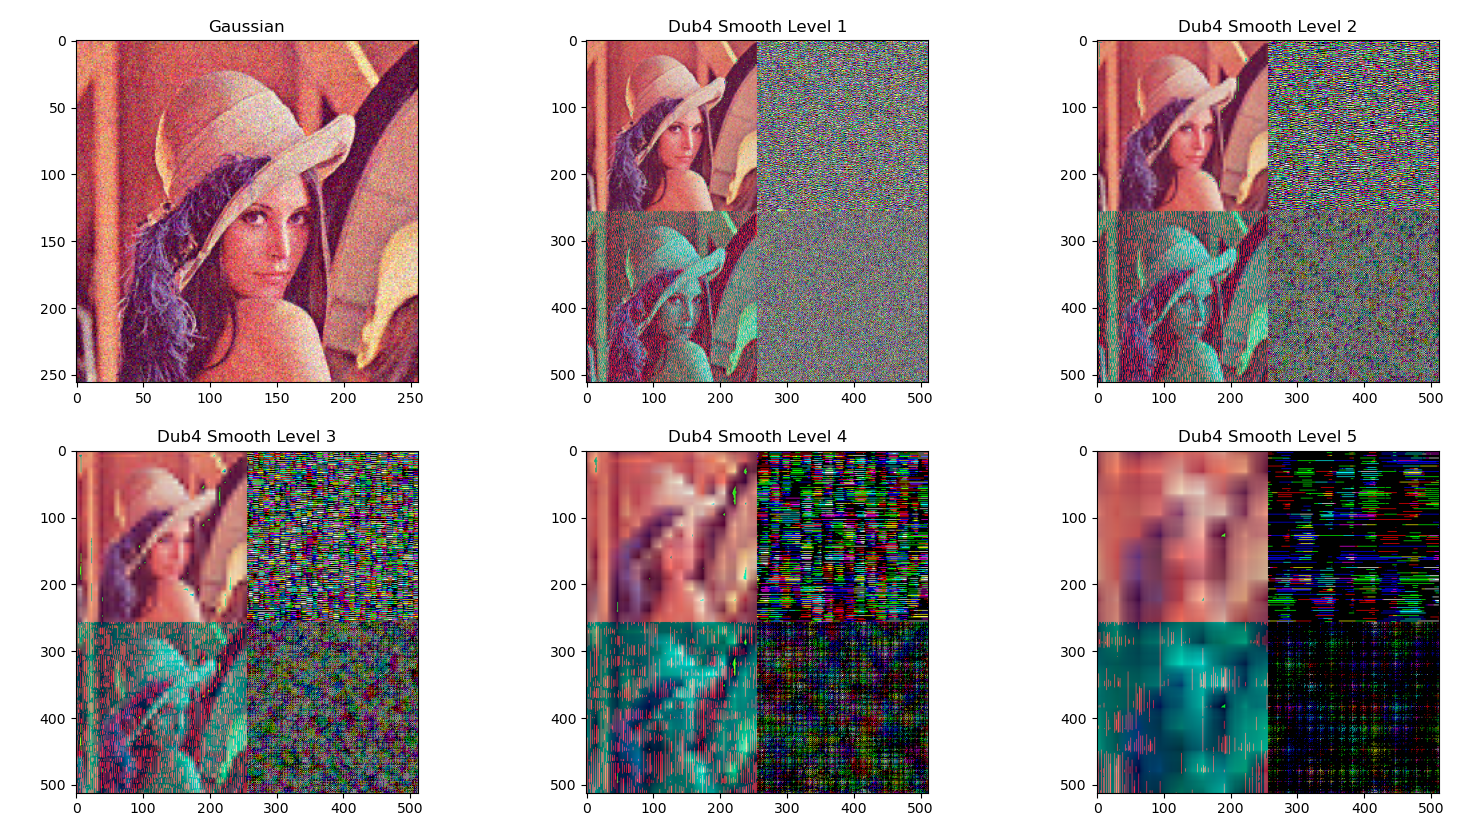
\includegraphics[width=0.8\textwidth]{img/Lena_Dub4.png}
    \caption{Daubechies4 2D Wavelet level1 to level5}
    \label{fig:mesh1}
\end{figure}
\subsection{Daubechies6 2D :}
\begin{figure}[h]
    \centering
    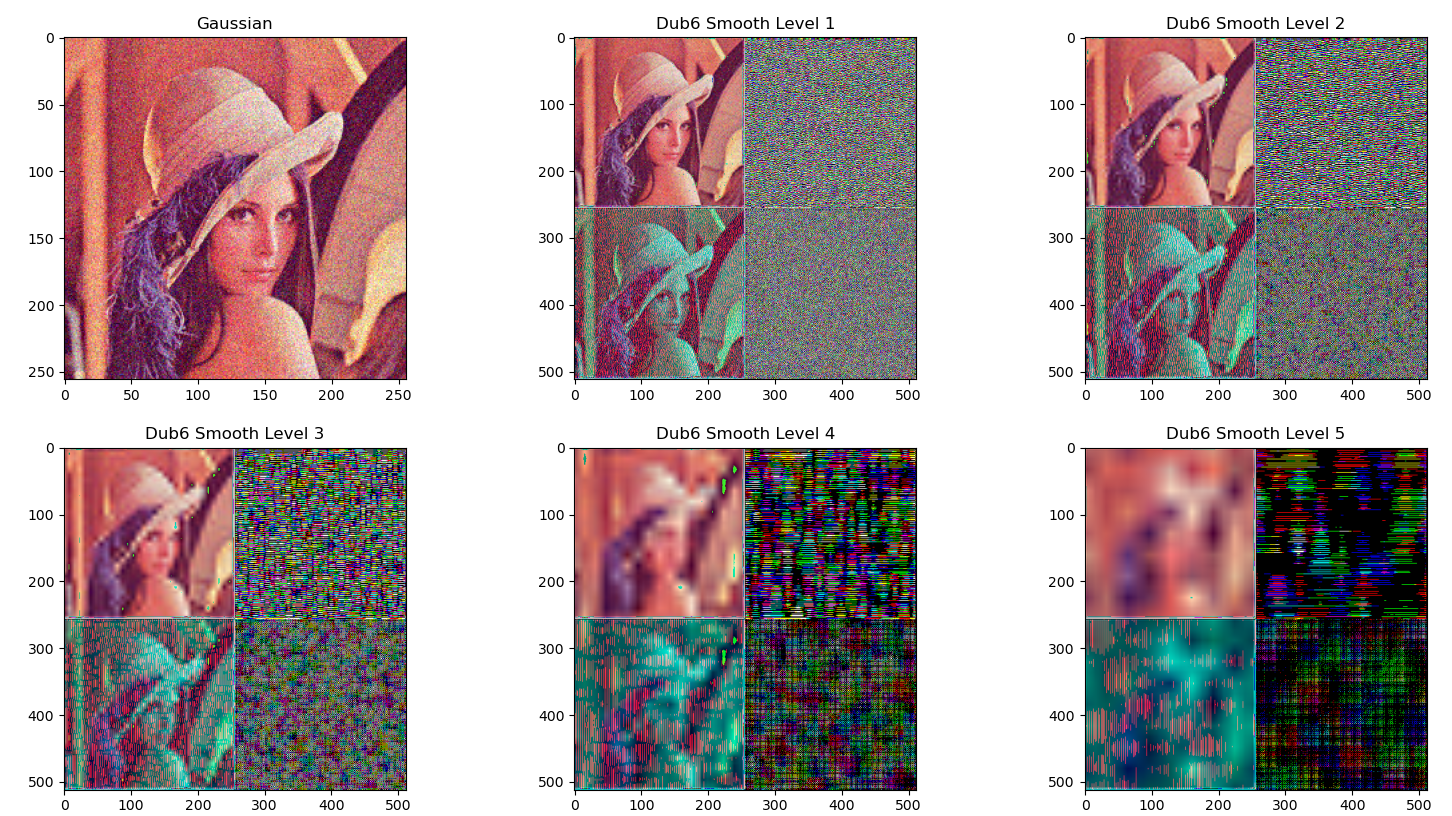
\includegraphics[width=0.8\textwidth]{img/Lena_Dub6.png}
    \caption{Daubechies6 2D Wavelet level1 to level5}
    \label{fig:mesh1}
\end{figure}
\newpage
\subsection{Mexician Hat 2D :}
\begin{figure}[h]
    \centering
    \includegraphics[width=0.8\textwidth]{img/Lena_Mex.png}
    \caption{Mexician Hat 2D Wavelet level1 to level5}
    \label{fig:mesh1}
\end{figure}

\end{document}